%-----------------------------------------------------------------------------
%
%               Template for sigplanconf LaTeX Class
%
% Name:         sigplanconf-template.tex
%
% Purpose:      A template for sigplanconf.cls, which is a LaTeX 2e class
%               file for SIGPLAN conference proceedings.
%
% Author:       Paul C. Anagnostopoulos
%               Windfall Software
%               978 371-2316
%               paul@windfall.com
%
% Created:      15 February 2005
%
%-----------------------------------------------------------------------------


\documentclass[]{sigplanconf}

% The following \documentclass options may be useful:
%
% 10pt          To set in 10-point type instead of 9-point.
% 11pt          To set in 11-point type instead of 9-point.
% authoryear    To obtain author/year citation style instead of numeric.

\usepackage{graphicx}
\usepackage{amsmath}
\usepackage{hyperref}
\usepackage{graphicx}

\newcommand{\squishlist}{\begin{list}{$\bullet$}
  {\setlength{\itemsep}{0pt}
    \setlength{\parsep}{3pt}
    \setlength{\topsep}{3pt}
    \setlength{\partopsep}{0pt}
    \setlength{\leftmargin}{1.5em}
    \setlength{\labelwidth}{1em}
    \setlength{\labelsep}{0.5em}}}

\newcommand{\squishend}{\end{list}}

\begin{document}

\conferenceinfo{Sprezzatech}{Aug 6, Atlanta.} 
\copyrightyear{2013} 
\toappear{Copyright is held by the author.\\
\textit{Sprezzatech} Aug 6, Atlanta.}
%\authorpermission
%\titlebanner{CS8803DC, Spring 2010, Georgia Institute of Technology}        % These are ignored unless
%\preprintfooter{Dynamic Translation for Intel's Loop Stream Decoder}   % 'preprint' option specified.

\title{Streaming Audio in the Gulf of Guinea}
\subtitle{The Psychoacoustics and Telecommunications of Nigeria}

\authorinfo{Nick Black}
           {nick.black@sprezzatech.com}

\maketitle

\begin{abstract}
Nigeria presents unique challenges and opportunities to mobile internet streaming
services. Major services such as Pandora\cite{pandoracountries} and
Spotify\cite{spotifycountries} have no presence in West Africa. Its multiethnic
and vivid culture produced worldwide sensations: Chinua Achebe, Wole Soyinka,
Chris Ofili, and ``Nollywood'', the hub of African cinema. Nigeria
was recognized as a ``Next Eleven'' country by Goldman-Sachs\cite{n11},
and is predicted by \textit{The Economist} to be the world's third most-populous
nation by 2050\cite{economist}. Cellular penetration approaches 70\% of the population\cite{nigeriamobile},
provides 70\% of the nation's internet access, and is expected to increase
dramatically following the dissolution and sale of the moribund, monopolistic
NITEL (Nigeria Telecommunications, Limited)\cite{reutersnitel}. This cellular access,
however, suffers reliability, quality-of-service, and capability issues, with
many users adopting multiple carriers\cite{reuterssims}. Furthermore, nascent
Nigerian streamers such as iROKING and Gbedu.FM have not introduced 
automated psychoacoustic categorization of African music. We investigate the
feasibility of cost-effective streaming and categorization of Nigerian music.
\end{abstract}

\category{ITU}{Region 1}{Nigeria}

\terms
Nigerian cellular, streaming music

\keywords
Nigeria, streaming, psychoacoustics

\section{Introduction}
The x86's CISC legacy, unique among modern processors, requires substantial
instruction decoding hardware and several pipeline stages. Recent Intel processors
provide no less than four instruction decoders, along with an MSROM. Of these,
only one (``complex'') decoder can handle instructions decoding to multiple
$\mu$ops; for very long instructions (those decoding to six or more $\mu$ops),
this complex decoder must engage the slow Masked-Or ROM unit and its
microcode store. This hardware's power requirements, not to mention the havoc
wrought on hot loops by front-end stalls, led to the introduction (on Crusoe
Core\texttrademark 2 processors) of the original Loop Stream Detector.
\\
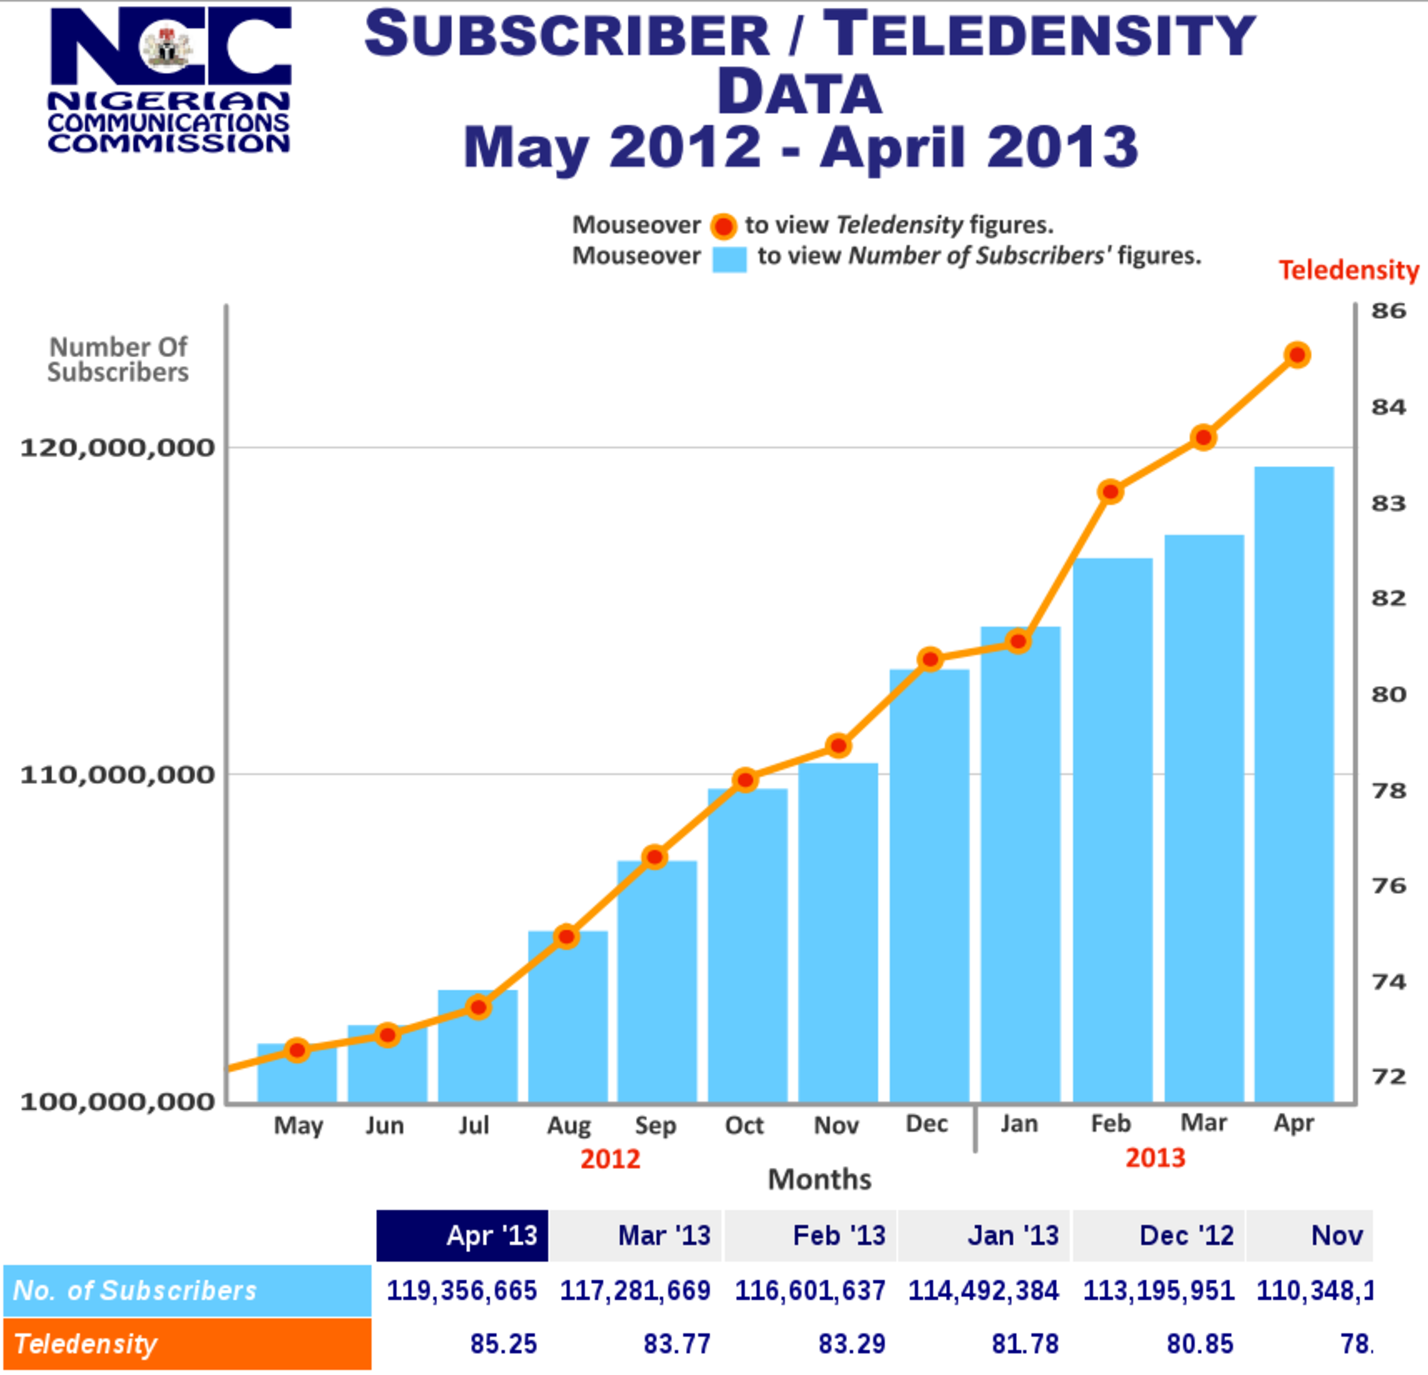
\includegraphics[width=\linewidth]{ncc.pdf}

%\begin{figure}[h]
%\includegraphics[width=\columnwidth]{texobjs/LSDConroe.jpg}
%\caption{The Core\texttrademark  2 Loop Stream Detector}
%\label{fig:lsdcorei7}
%\end{figure}

Benefits of the original LSD included \cite{inteloptimize}:
\squishlist
\item The documented ability to shut down instruction fetch and branch prediction hardware.
\item The possibility of shutting down instruction cache \textit{in partes} or
\textit{in toto}, as explored in other processor designs \cite{badulescu} (no
such capability has been mentioned in Intel documentation).
\item Elimination of delays due to misaligned branch targets.
\item Recovery of execution bandwidth used by branch instructions.
\squishend

The Loop Stream Detector was improved for the release of the ``Nehalem''
Core\texttrademark i7. Moved after the decoding stages, it now supplies $\mu$ops directly
to execution units (as opposed to instructions to the decoder).

%\begin{figure}[h]
%\includegraphics[width=\columnwidth]{texobjs/LSDCorei7.jpg}
%\caption{The Core\texttrademark  i7 Loop Stream Detector}
%\label{fig:lsdcorei7}
%\end{figure}

Benefits include:
\squishlist
\item The entire processor frontend can be powered down during LSD streaming,
as opposed to merely the instruction fetching hardware.
\item Length-Changing Prefix stalls, major sources of delays in the frontend,
are eliminated.
\item Stalls due to contention for the single complex instruction decoder are
avoided, as are the extreme delays due to MSROM-based decoding.
\squishend

The Loop Stream Decoder is a microarchitectural property: it operates wholly
without programmer intervention, and is not visible in the x86 ISA. The LSD
will cache any instruction/$\mu$op stream that has looped (branched backwards)
64 times, and meets the following conditions:
\squishlist
\item It requires no more than 4 instruction fetches of 16 aligned
bytes each.
\item It contains no more than 4 branches, none of them a CALL or RET.
\item It contains no more than 18 instructions (on Core\texttrademark 2).
\item It contains no more than 28 $\mu$ops (on Core\texttrademark i7).
\squishend

\section{Optimizing for the LSD}
Optimizing for the LSD requires the abilities to recognize hot loops, determine
whether or not a given loop is suitable for the LSD, and transform unsuitable
loops into suitable forms. This last must be performed while honoring the
original program's semantics, and (obviously) in a fashion guaranteed to
terminate. Daytripper leverages the DynamoRIO binary translation framework
for disassembly and encoding of instruction streams, and its \textit{trace}
objects (as opposed to \textit{blocks}) provide suitable recognition of hot
loops.

\subsection{Determining LSD suitability}
Determining whether or not a loop qualifies for the LSD can be a difficult task
in and of itself. The requirements of the Core\texttrademark 2's LSD are simple
enough for a static compiler to consider, but the Core\texttrademark i7's LSD
complicates matters by caching $\mu$ops rather than instructions. Intel does
not (at this time) make public the correspondence of instructions to $\mu$ops\footnote{Agner Fog's venerable datasheets \cite{agnerfog} do publish an approximate correspondence, but these follow processor releases, at best, by several months.}. These 
mappings change from processor to processor or even stepping to stepping, and
are further mudded by microarchitectural techniques such as Micro- and Macro-fusion. Any
compiler must already have some idea of $\mu$op mappings
if it is to fully optimize for decoder resources, but simply knowing which
instructions decode to multiple $\mu$ops is sufficient to make full use of
Pentium-M, NetBurst, Core and Nehalem microarchitectures' ``3-1-1'' or ``4-1-1-1''
decoder arrangements.

Thankfully, a performance monitoring counter (LSD\_UOPS, event 0xA8) was
introduced alongside the improved LSD. While a static compiler (especially in
the absence of profile-guided optimization) would be hard-pressed to
effectively make use of this PMC as a litmus (especially as runtime code
placement decisions can affect suitability), a dynamic compiler is well-suited
to begin its search with the counter. Daytripper simply resets the counter on
entrance to a DynamoRIO trace entry callback, and checks it during the trace
exit. If the counter has changed, the LSD has been employed, and Daytripper
needn't perform further work. Likewise, a zero count suggests analysis of the
associated trace.

The performance counter also serves to gauge our effectiveness. Daytripper
marks any trace it modifies. Since it never transforms a trace which triggered
the LSD, any marked trace with a non-zero LSD count represents a successful
transformation\footnote{This doesn't hold if DynamoRIO itself triggers the LSD.}. Other marked traces represent wasted work, and are indicative
of bugs in Daytripper's suitability testing. Given this instant and highly
accurate feedback, any errors in $\mu$op mapping ought be flushed out quickly.
Daytripper is thus fairly resilient against microarchitectural changes\footnote{The
author spent significant time planning integrating such a scheme into GCC's PGO, thinking
it the coolest part of this project.}, or at least automatically discovers any
which affect its effectiveness. Furthermore, this allows binaries to be
sorted based on whether they can effectively be transformed (subject, of course,
to the same vagaries which complicate static PGO). Daytripper translation can
thus be foregone when it will have no effect.

Verifying other properties is a fairly simple (if distinctly unpleasant) task.
This merely requires knowledge of branch instructions (at the ISA level) and
their LSD limits, location of the code at runtime, disallowed instructions,
and properties of the instruction fetch unit. These last are microarchitectural
properties, but thankfully not a maintenance burden: the CPUID instruction
allows all relevant properties (page size, instruction cache size, and
associativity)\footnote{Whether the instruction and data caches are unified is irrelevant;
we're verifying not residency, but boundary crossings.} to be discovered
at runtime.

\subsection{Extracting LSD suitability}
Transformation, as could be expected, is the most complicated aspect of
Daytripper's operation. More correctly, transformation \textit{will be} the
most complicated aspect; Daytripper, originally a static binary translator,
was reinvented as a dynamic tool very recently. Such transformations are, for
all intents and purposes, beyond the capability of a static x86 translator.
The ubiquity of indirect branches (even discounting clear linker patch-up points,
as can be determined via cross-referencing ELF's \texttt{.plt} section) would
be sufficient to exclude most transformations\cite{landi}; the x86's variable
instruction length, relaxed alignment requirements for execution and access,
and support for self-modifying code quickly render the problem intractable,
if it is indeed even decidable.

\section{Loop size reduction}

For each requirement of the LSD, there exists a corresponding class of
transformations we might perform. Many of them would already have been
executed by a reasonable static compiler, and thus we oughtn't expect them
to be exploitable in optimized code. This will be of critical importance
when selecting benchmarking tools; it'll likely be best to build up a unit
testing infrastructure around small, hand-written assembly snippets.

\subsection{Code requires more than 4 fetches.} First, ensure that the loop is
properly aligned (this will generally be true for optimized code). Otherwise,
attempt loop size reduction as outlined in section 3.3. Note that instructions
must be minimized in 3.3, even if the LSD is $\mu$op-based; it might thus be
necessary to minimize \textit{both} $\mu$ops and instructions on Core\texttrademark i7
processors and later.

\subsection{Code contains more than 4 branches.} Attempt to replace branches with
predicated instructions. Daytripper is only active on processors with Loop
Stream Detectors, all of which include the P6-era \texttt{CMOVxx}; it is thus
safe to conditionalize where possible (it is unfortunate that x86 is not a more
fully predicated instruction set, such as ARM \cite{seal} or IA64). This transformation is
unlikely to slow down the loop body, and thus again we can expect optimized
code to already have used \texttt{CMOVxx} where applicable. Compilers
optimizing for size or speed, however, are unlikely to use certain
bit-parallelism tricks \cite{warren} we might exploit, especially in highly
idiomatic arithmetic loops. This might be fertile ground for future research.

\subsection{Code is too large} For Core\texttrademark 2, or to reduce the number
of necessary fetches (see 3.1), we seek to minimize instructions. For Core\texttrademark i7
and beyond, we seek to minimize $\mu$ops. These goals are not incompatible,
but neither can they generally be achieved via the same transformations.
Unoptimized code can of course be easily shrunk, but we assume reasonable
optimization for space---in which case we are unlikely to achieve much
reduction---or speed, which has as its most basic heuristic ``minimize dynamic
instructions''. Once again, however, we can perform some ``regressive transformations''
which possibly sacrifice performance.

Whether to do so must be decided considering the benefits of the Loop Stream
Detector. Loops containing length-changing prefixes, for instance, incur weighty
stalls in the decoding logic. By bypassing the decoders (on Core\texttrademark
i7), the LSD may well effect a net speedup even as it undoes other optimizations.
These stalls have long been known to the compiler-writing community, so it is
unlikely that they're generated in any real abundance. If code were found that
had been forced to incur LCP stalls so that some other powerful optimization
could be performed, Daytripper could unleash potent performance gains indeed.

``Magic divisions'' trading size for speed \cite{knuth2} could be replaced
with their equivalent constant divisions. \texttt{ADD}/\texttt{SUB} $\#-1$ instructions
could be replaced with their equivalent \texttt{INC}/\texttt{DEC}s, especially
if the condition register-carried dependencies these instructions introduce
were demonstrated to be innocuous (perhaps by introducing a dependency-breaking
instruction). Sets of \texttt{PUSH}es and \texttt{POP}s, used
to minimize the number of stack writes, could be replaced with a single
\texttt{PUSHA}/\texttt{POPA} pair. This is unlikely to affect performance negatively,
due to a large ratio of cacheline to word lengths (it ought be noted, however,
that these are $\mu$op-intensive instructions). In any case, extensive pushing
and popping is unlikely to occur in a hot, reasonably-optimized loop.

If the 4-fetch limit is not close to being breached (in an extreme case, 18
single-byte instructions), a counter-intuitive method would be to eliminate
internal NOPs present only for alignment purposes. Since the LSD eliminates
misaligned instruction penalties, these NOPs have no purpose in a loop
streamed from the LSD.
\section{Related work}
Virtually every reference to the Loop Stream Detector, from GCC bug reports
\cite{gcclsd} to various optimization guides, speaks of supposed performance benefits.

This is wrongheaded.

While it is true that streaming instructions (in the case of Conroe) or $\mu$ops
(in the case of Nehalem) from the Loop Stream Detector bypasses several pipeline stages,
this does not, by itself, represent a gain in throughput. At a saturated steady
state, IPC is independent of pipeline length. The LSD applies only to tight
loops---precisely the sections most easily benefited by branch prediction,
large data caches, advanced prefetching and extensive speculation. In short,
it targets code for which Intel has already spent a decade adding hardware
support (as noted earlier, the LSD \textit{can} remedy certain decoding
perversions specific to the x86 architecture).

The LSD would be highly relevant to research on optimizing for power, were it
not for the facts that:
\squishlist
\item It is present only on energy-hungry high-end x86 processors, poor fits for
systems designed to conserve power.
\item It is only so effective at reducing power consumption due to the large
transistor budget required for high-speed x86 instruction decoding; a classic
RISC processor could not reap nearly such significant benefits.
\squishend
Whether or not the Loop Stream Detector will emerge as the focus of academic
research is debatable. This paper appears to be the first investigation
of dynamic translation for the explicit purpose of engaging the LSD.
\appendix
\section{Using the LSD\_UOPS PMC}

\bibliographystyle{abbrvnat}
% The bibliography should be embedded for final submission.
\bibliography{nigeria}
\end{document}
